\chapter{Introduction}\label{ch:1}

\epigraph{Any fool can write code that a computer can understand. Good
programmers write code that humans can understand}{Martin Fowler}

\section{Motivation}
	We all want to write quality code. Code that follows the company standards,
that has an amount of test coverage, that does not use system hack, etc. In
order to be able to measure and enforce this characteristics we need to use software
analysis tools such as:
	\begin{description}[labelindent=2cm]
	\item[Wala Tool]  Developed by IBM Research it implements a series of dataflow
and type analysis algorithms.
	\item[FindBugs]   Widely used tool to detect common programming language hacks
	\item[Intellij IDE] {A platform developed by JetBrains which implements over
100 code inspector tools}
	\item[CodePro]   A platform which implements software metrics developed by
LOOSE Research Group. Goes by the name of INCODE, also \cite{tools:inCode}
	\end{description}

	Of course there are many more tools such as the ones provided. These are only
some of the most used ones.
	
	In order for the software analysis tools to be able to analyse the code they
need a metamodel. A metamodel represent all the elements necessary to describe a
model, in our case all the elements necessary to describe the code, i.e the
classes from a program, the methods from the classes, the fields from the
classes \ldots{} etc.
	Consider the situation in figure \ref{fig:metamodels}

\begin{figure}
\centering
\scalebox{0.5}{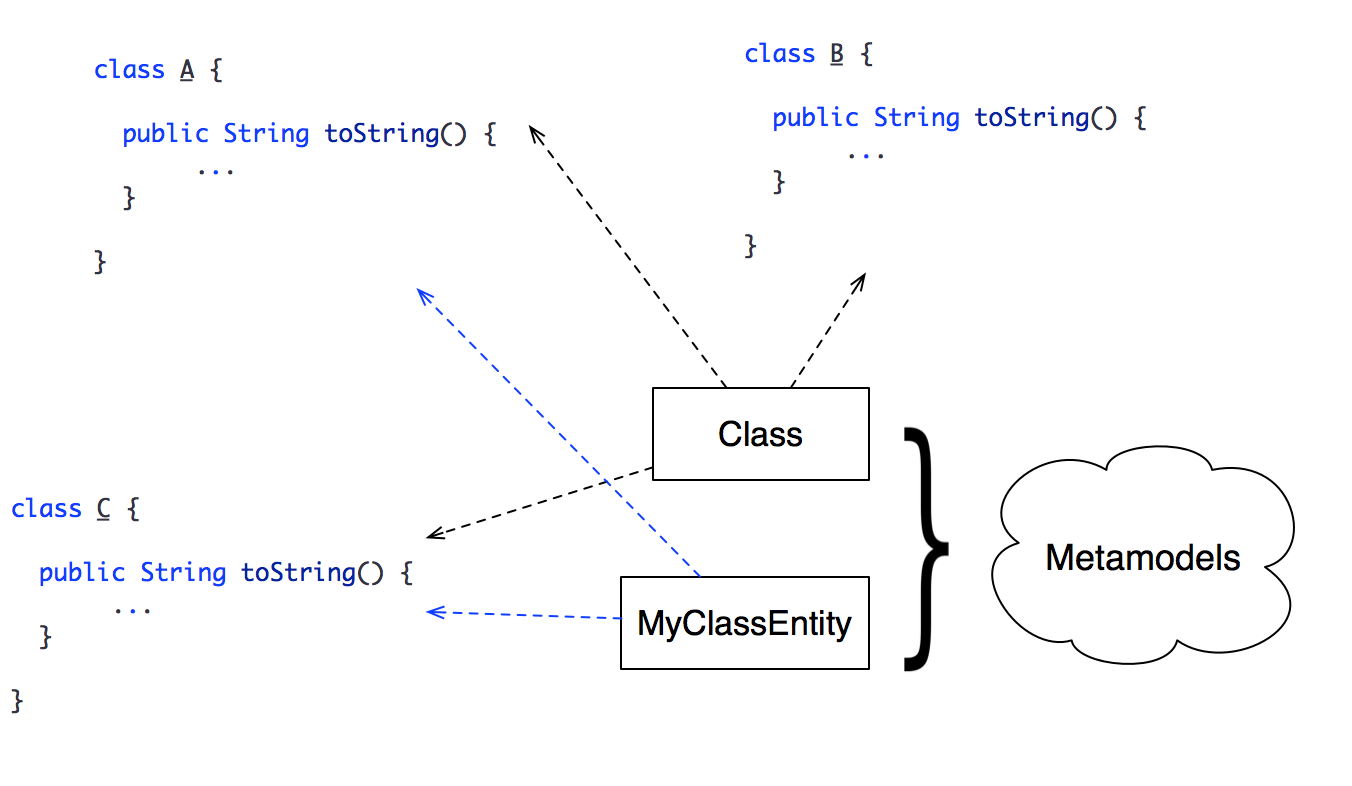
\includegraphics{../img/introductions/Metamodels.png}}
\caption{Two different metamodels for the same model}
\label{fig:metamodels}
\end{figure}	
	
	We have two valid metamodels that describe similar elements, but they cannot be
integrated. If we want to build an easily extensible and integratable platform
for tools we need more than a metamodel, we need a meta-metamodel. CodePro has
such a meta-metamodel. In figure \ref{fig:codeProUml} we can see a glimpse of
CodePro meta-metamodel and how easy it is to add new metrics. We only have to
extend the  \code{PropertyComputer} class
	
\begin{figure}
\centering
\scalebox{0.5}{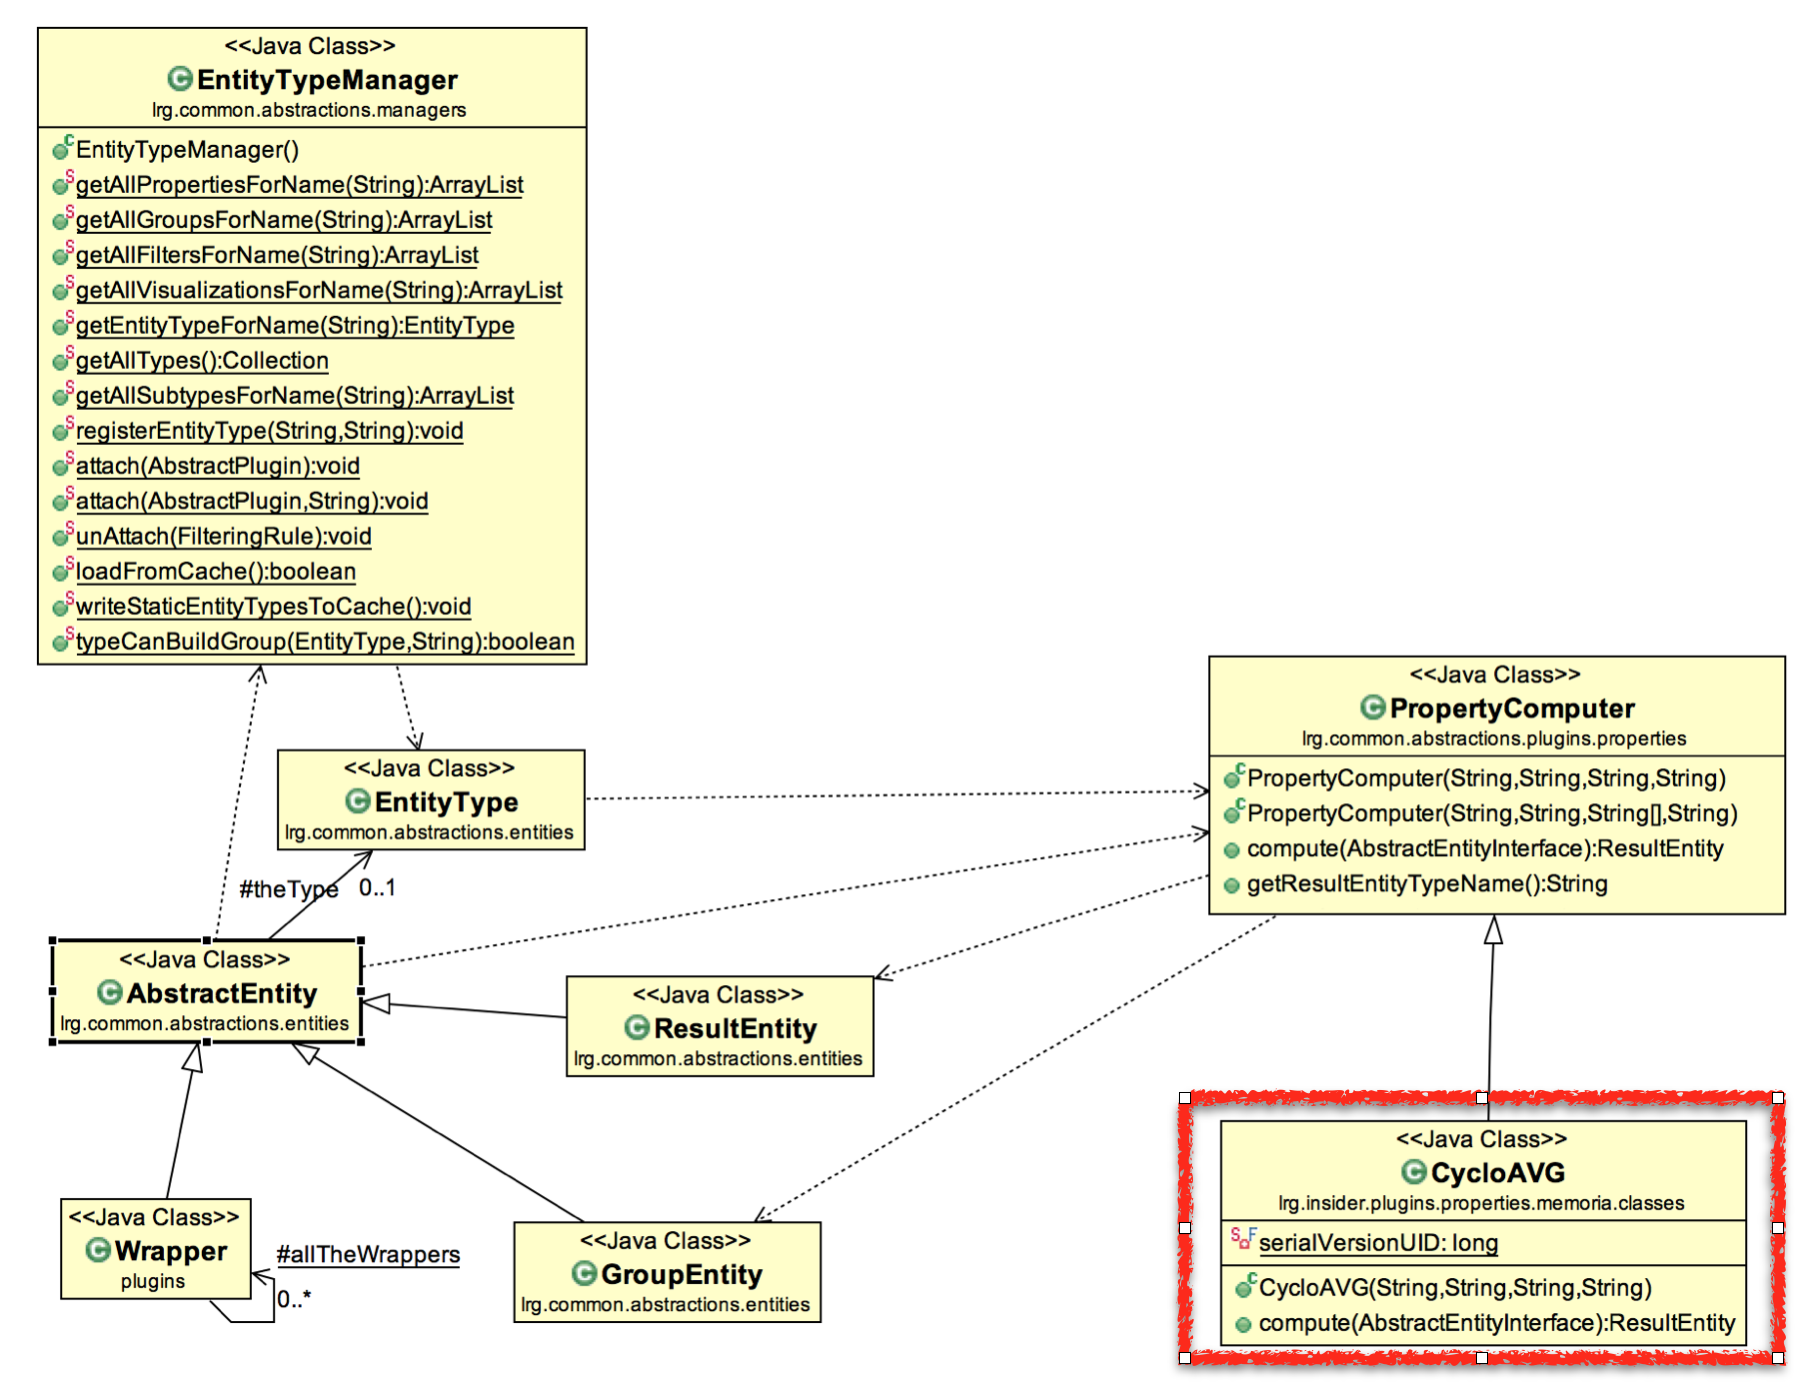
\includegraphics[angle=90]{../img/introductions/CodeProUML.png}}
\caption{CodePro UML}
\label{fig:codeProUml}
\end{figure}

	Unfortunately with the desire of extensibility some architectural design
problems where introduced which breaks statically type safety and make it harder
to understand and maintain the code. In figure \ref{fig:CycloAVGCodePro} we
can see an example of metric written in CodePro. With red I've marked the major
problems for which we will present a solution. We can see that there are alot of
magic constants present in the code. These magic constants are used to identify
the tools in the system. From this a simple problem arises: What if we the id
(e.g CYCLO) changes or we misspelled it ? Another problem is the generic
\code{AbstractEntityInterface} which denotes every element from the metamodel.
What would happend if for the Cyclomatic Complexity metric we pass a class
entity instead of a method entity ? The answer to both the questions is simple,
if we are lucky at runtime the application will throw an exception. Basically we
managed to become \textbf{dynamically typed} even if we are programming in a
statically typed language.

\begin{figure}
\centering
\scalebox{0.4}{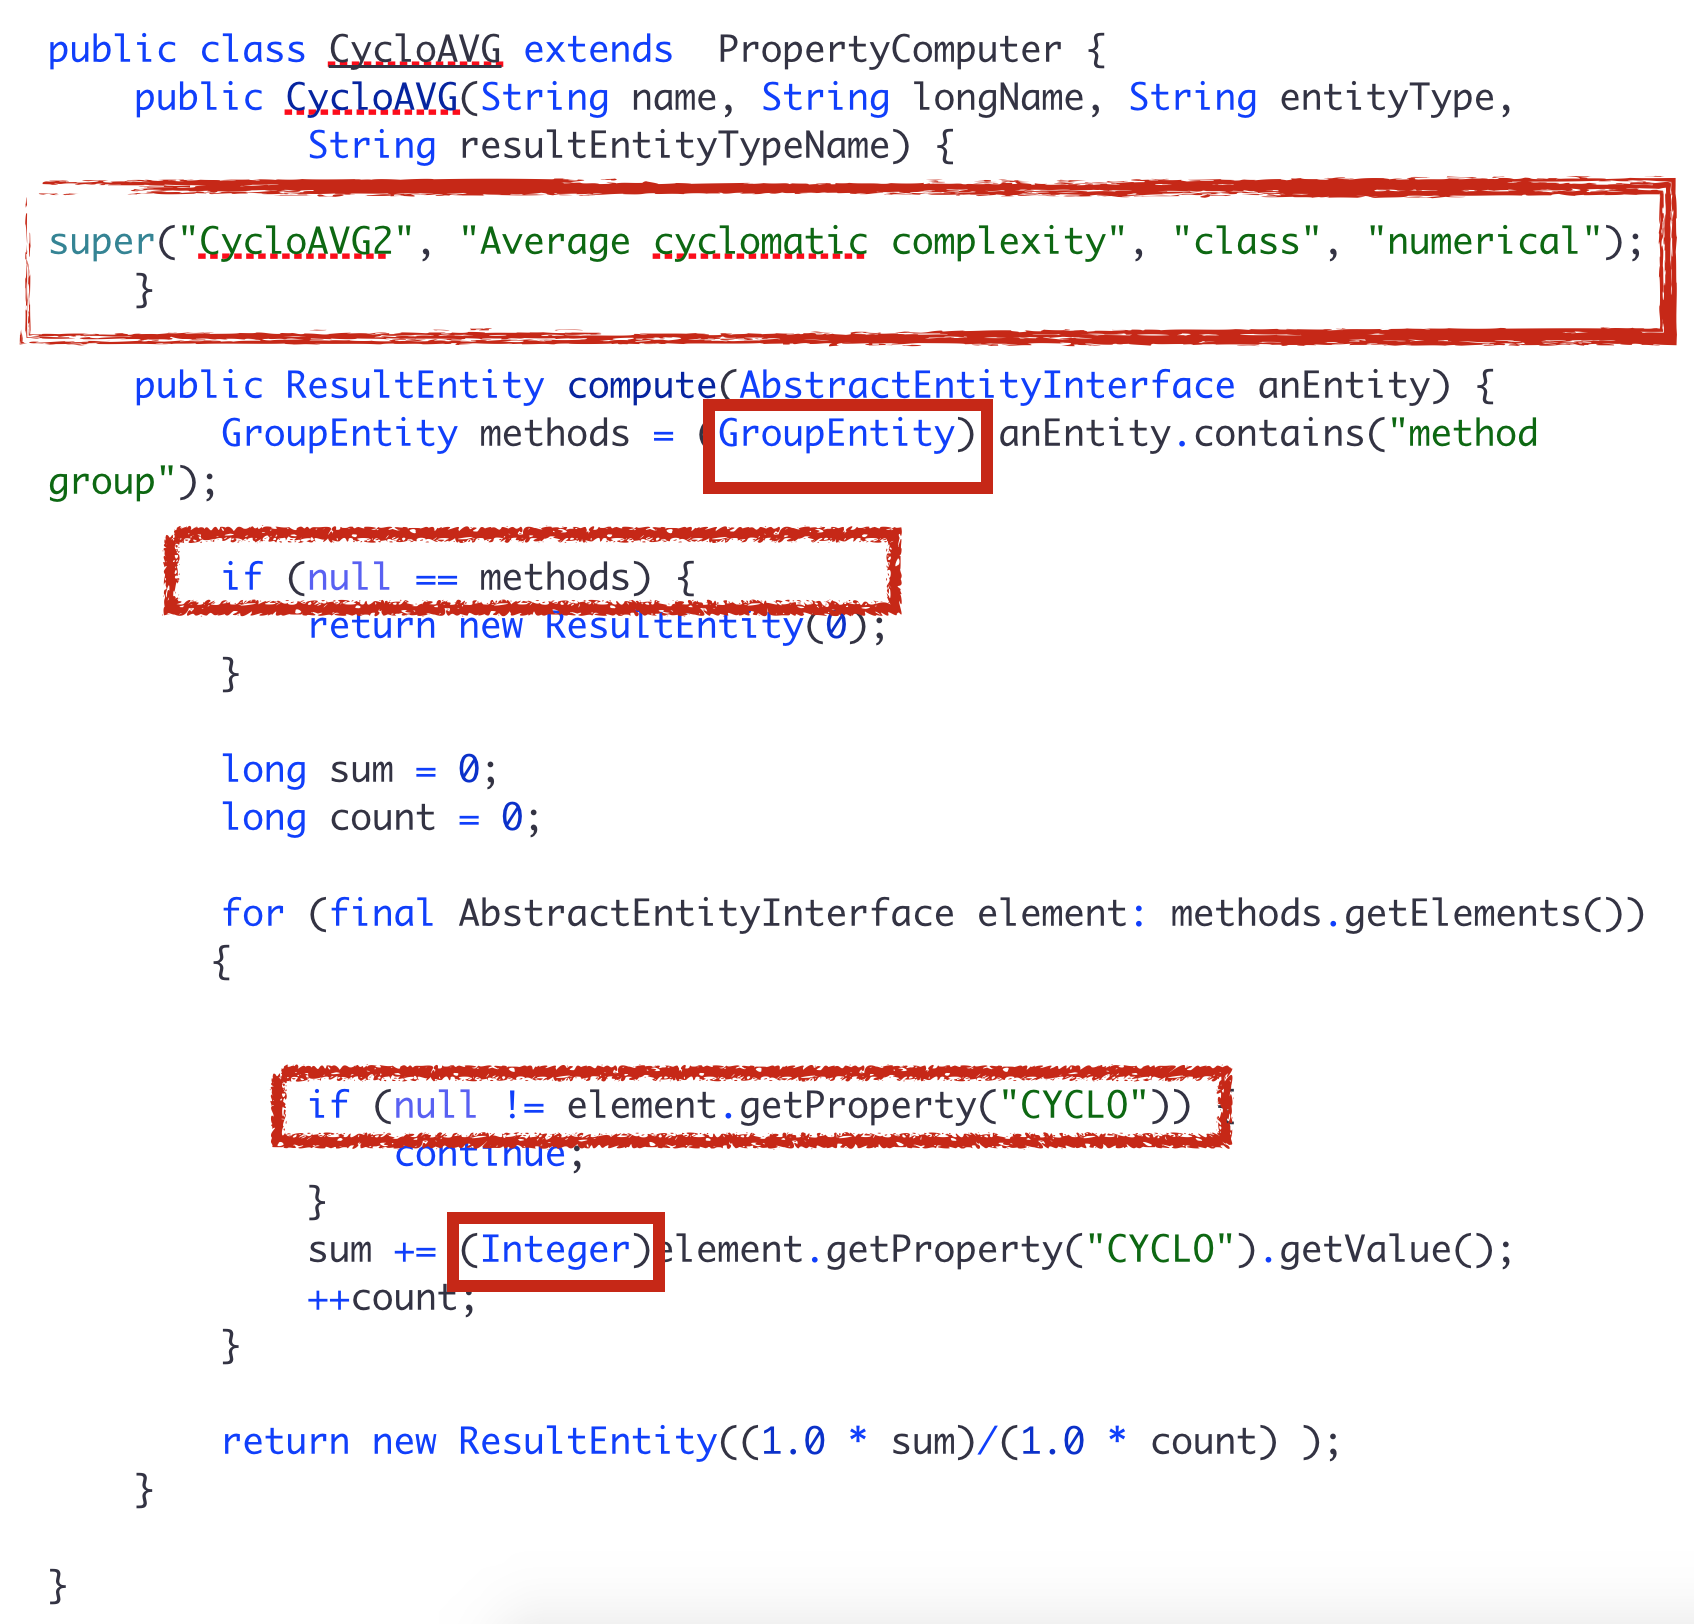
\includegraphics{../img/introductions/CycloAVGCodePro.png}}
\caption{CodePro UML}
\label{fig:CycloAVGCodePro}
\end{figure}

\section{Goals and Contributions}
	
	Our purpose for this thesis is to present a solution for the problems presented
in the previous section. We want to become \textbf{statically typed} again and
also be easily extensible and integratable. We shall present an innovative tool
called XCorex which can solve the problems. XCore provides a flexible implementation of a meta-model. 
The user can provide any number of plugins (e.g. metrics implementations) 
that are annotated in terms of the provided meta-metamodel. XCore processes the
user annotations and automatically and seamlessly produces  the Java code of the metamodel and
the required link between the metamodel properties (e.g., metrics) and their implementation (e.g., plugin).
Finally, since these metamodel is expressed in terms of Java classes, 
invoking a model property will be safe (because it will be checked by the compiler). 


\section {Organization}
		Chapter 2.  A thorough presentation of the fundamental concepts that are going
to be used in this work in order to avoid any ambiguities.	It will cover
elements regarded eclipse plugin development, meta-metamodeling, metamodeling,
modeling and how they can be implemented in Java. Also we present a state of the
art analysis tool CodePro and detail the problem we are solving.

	Chapter 3.  The anatomy of XCore will reveal the solution we purpose for the 
problem. All mechanisms that allow the framework to work as intended (ease of
use and extensibility) will be explained in details.  Also we introduce a tool
that I have implemented in order to properly evaluate the tool and the actual
evaluation.
	
	Chapter 4.  In this chapter we summarize all the information described in
previous chapters and present the conclusions. Also, I present the future work
which will be done in the development process of the tool.	
	